\documentclass[10pt]{article}

%%% These are some packages that are useful
\usepackage{amsmath,amssymb, amscd,amsbsy, amsthm, enumerate}
\usepackage[export]{adjustbox}
\usepackage{lastpage}
\usepackage[top=1in, bottom=1in, left=1in, right=1in]{geometry}
\usepackage{tikz, pgfplots, xcolor, fancyhdr}
\usepackage{multicol}
\usepackage{lipsum}

%%% Page formatting
%\setlength{\headsep}{30pt}
\setlength{\textheight}{9in}
\newcommand{\tab}{\hspace{1cm}}
%\setlength{\parindent}{25pt}

\title{A Lion In A Cage}
\author{Antonius Torode}

%%% Header and Footer Info
\pagestyle{fancy}
\fancyhead[L]{{\large Template - \textbf{Change 03}}}
\fancyhead[C]{\today}
\fancyhead[R]{Name: Antonius Torode}


\fancyhf{} % sets both header and footer to nothing
\renewcommand{\headrulewidth}{0pt}
% your new footer definitions here

\fancyfoot[L]{}
\fancyfoot[C]{}
\fancyfoot[R]{\thepage\ of \pageref{LastPage}}

% Used to define spacing and format of References
\let\OLDthebibliography\thebibliography
\renewcommand\thebibliography[1]{
	\OLDthebibliography{#1}
	\setlength{\parskip}{0pt}
	\setlength{\itemsep}{0pt plus 0.3ex}
}

%%% Document Starts now
\begin{document}

\maketitle
\thispagestyle{fancy}

%\begin{abstract}
%	This message explores the contrast between the natural freedom designed by God and the seductive promises of worldly comfort. Using vivid allegory, it follows the life of a lion - once wild and free but later domesticated and caged. This example highlights how ease, safety, and provision can subtly lead to dependency and loss of purpose. Through scripture and reflection, it warns against trading autonomy and spiritual vigilance for the illusion of security. The message calls readers to remain steadfast, to resist societal pressures, and to rediscover truth and perspective through the wisdom of God’s creation.
%\end{abstract}

\begin{multicols}{2}


Consider the lilies of the field, how they grow: they neither toil nor spin\footnote{Matthew 6:28: ``So why do you worry about clothing? Consider the lilies of the field, how they grow: they neither toil nor spin;''}. Look at the birds of the air, for they neither sow nor reap nor gather into barns; yet your heavenly Father feeds them\footnote{Matthew 6:26: ``Look at the birds of the air, for they neither sow nor reap nor gather into barns; yet your heavenly Father feeds them. Are you not of more value than they?''}. But now ask the beasts, and they will teach you; And the birds of the air, and they will tell you; Or speak to the earth, and it will teach you; And the fish of the sea will explain to you\footnote{Job 12:7-8: ``But now ask the beasts, and they will teach you; And the birds of the air, and they will tell you; Or speak to the earth, and it will teach you; And the fish of the sea will explain to you.''}. God gave us nature so that we may learn from it.

\begin{center}
	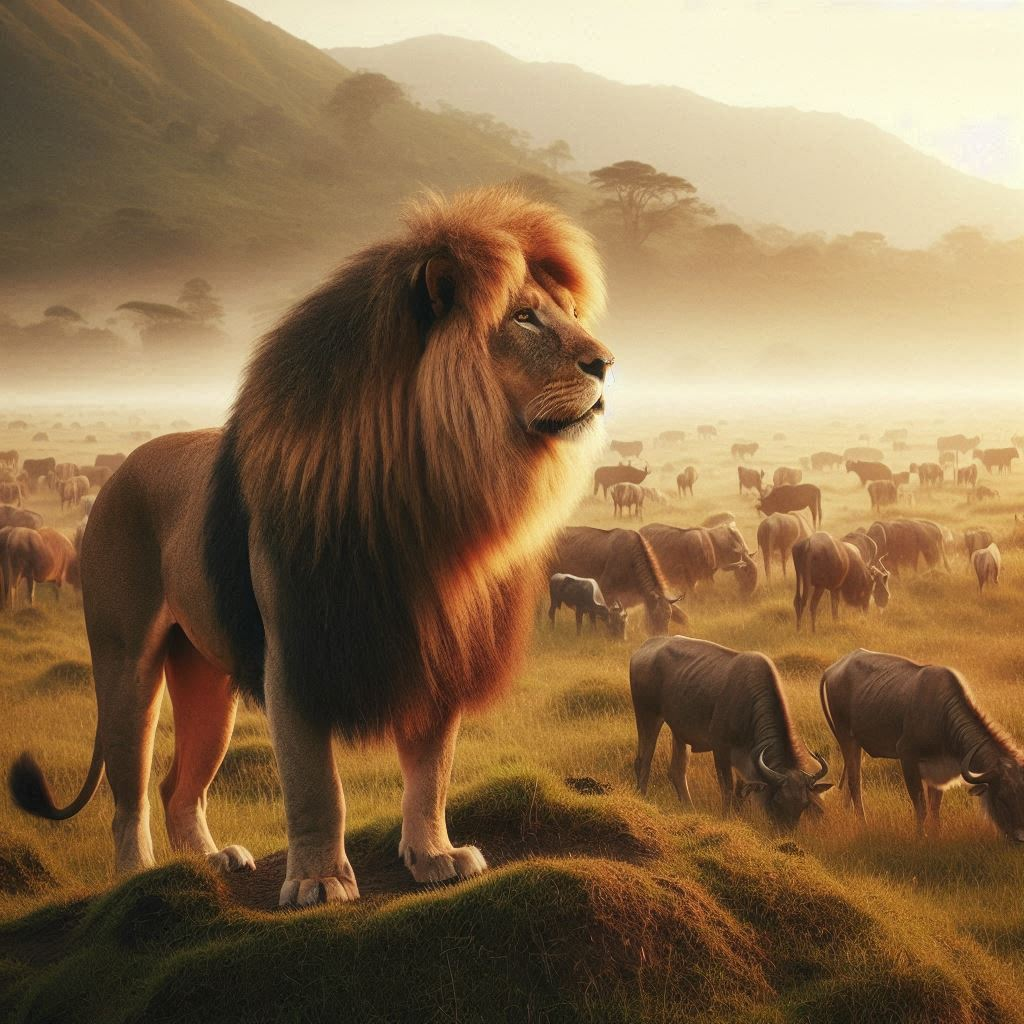
\includegraphics[width=0.48\textwidth]{lion.jpeg}
\end{center}

Imagine for a moment, that you are a lion, living out in the wild Savannah. When you're hungry, you hunt some of the local prey. You've never died of hunger - there's food to hunt for all over. The trees provide you with fresh fruit and the fields with fresh herbs. When you're tired, you lay under the vast stars of the heavens. You can wander to and fro, far and wide, seeing the beautiful sights that nature has to offer. When you're ready to relax, you have the sounds of the birds chirping around you, the gentle breeze in your mane, and the streams and waterfalls flowing around. Life is good... right?

One day a pack of hyenas comes around and starts bothering you. When you turn your back, they steal the food you hunted for. If you drop your guard, they may even try to eat \textit{you}. You begin to realize it's not as safe as you thought. One day, the sun burns bright. The heat makes you tired and weak as the sun burns on your skin. Another day, rain comes and stays for days on end. Your pelt stays wet and refuses to dry. You realize that you don't quite have the shelter you need. One day you don't manage to catch the prey you chased. You're tired and weak, you haven't eaten in days. You begin to realize that hunger is not a very fun feeling. If only you had some food, life would be good again. You then see a snake. As hungry as you are, you go after it, only to come away with a paw full of venom. The fangs were sharp and piercing - now a constant stinging. If only you had a doctor, life would be good.

Along comes a man. He looks at the struggles you have and makes you an offer which sounds too good to be true. ``Little lion, how would you like free food? I can feed you promptly each day. How would you like free shelter? I can give you a solid roof over your head. How would you like free security? I can keep all of the hyenas from pestering you. How would you like free healthcare? I can take care of your paws every time you step on a spike. All this for you, for free.'' You may wonder what the catch is. For beware lest anyone cheat you through philosophy and empty deceit, according to the tradition of men\footnote{Colossians 2:8: ``Beware lest anyone cheat you through philosophy and empty deceit, according to the tradition of men, according to the basic principles of the world, and not according to Christ.''}. But there's no catch - he's offering exactly what he says he is. Of course, you accept the offer! With all these things, life will be great!

And so sure enough, everyday you are handed free food. The hyenas no longer sneak around when you're not looking. The sun no longer burns on your skin and the rain no longer keeps you wet for days. So you say `I have become wealthy, and have need of nothing'\footnote{Revelation 3:17: ``Because you say, ‘I am rich, have become wealthy, and have need of nothing’—and do not know that you are wretched, miserable, poor, blind, and naked''}. You realize now that life will be truly good - better than ever before. Little do you realize that you are wretched, miserable, poor, blind, and naked\footnotemark[\value{footnote}].

After a short period of time, you begin to tire of the same meal each day. You miss the thrill of the hunt. You miss the freshness of the food. You realize that your legs are weakening as you no longer wander to and fro. All you do now is lay around. You begin to miss the relaxing peace of sitting in the rain or bathing in the sun. One day you roll over and lay on your back to relax, only to realize... the stars are gone. The birds no longer chirp. The waterfalls no longer flow in the distance. You look around and wonder, where are you? You realize that you are now living in a cage. 

\begin{center}
	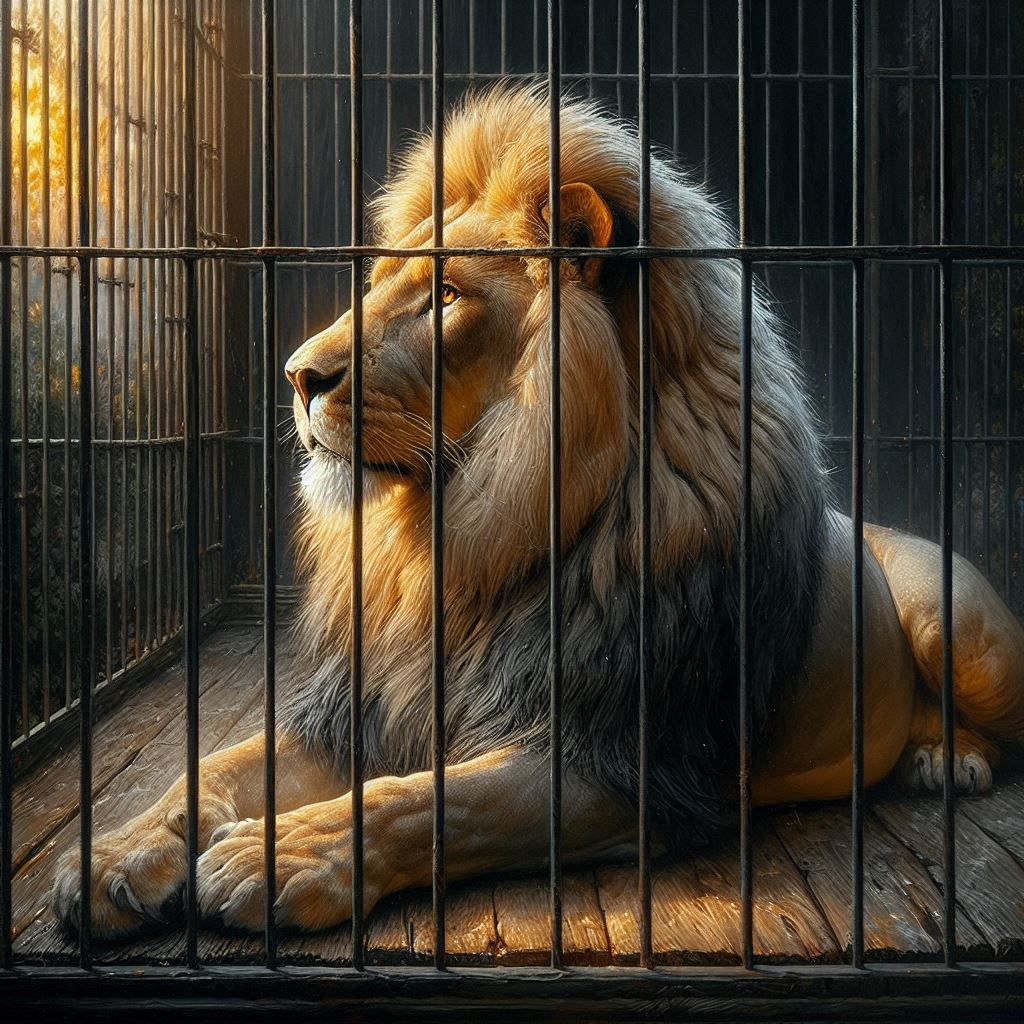
\includegraphics[width=0.48\textwidth]{cage.jpeg}
\end{center}

From your cage you can no longer see the lilies of the field. You can no longer hear the birds of the air. The beasts of the field are no longer available to teach you. The fish can no longer explain to you. All of these things were taken from you without you knowing. But how did this happen? The man who offered you comforts and freedoms technically spoke the truth - and you accepted it willingly. At the time you didn't hear it for what it was. For when they speak great swelling words of emptiness, they allure through the lusts of the flesh\footnote{2 Peter 2:18-19: ``For when they speak great swelling words of emptiness, they allure through the lusts of the flesh, through lewdness, the ones who have actually escaped from those who live in error. While they promise them liberty, they themselves are slaves of corruption; for by whom a person is overcome, by him also he is brought into bondage. ''}. And no wonder! For Satan himself transforms himself into an angel of light. Therefore it is no great thing if his ministers also transform themselves into ministers of righteousness\footnote{Corinthians 11:14-15: ``And no wonder! For Satan himself transforms himself into an angel of light. Therefore it is no great thing if his ministers also transform themselves into ministers of righteousness, whose end will be according to their works.''}.

All too often, we fall into struggles that make daily life just that much harder. When the hyenas inevitably come out of nowhere to pester us, we cannot allow ourselves to lose perspective. These are the subtle moments that shape how we see the world. Without darkness, we don't see the light as clearly. Without the occasional storm, how are we to truly appreciate the clear days? Struggles, frustrations, and hardships are not something we can bend a knee to. We are called not to give up - but to overcome. But society and the ministers of Satan count on pushing us past our levels of comfort. We see it time and time again. Satan tempted Eve in the garden of Eden. He whispered to her that his way would be better. Esau gave up his birthright for a single meal. The Israelites yearned to return to Egypt. Even today, entire countries give up their freedoms in exchange for the promise of safety, convenience, or stability. People willingly accept surveillance in exchange for security, censorship in exchange for peace, and dependence in exchange for equality.

So, when the men of the world come to you with offerings of free comforts, be cautious. When Satan tempted Jesus in the wilderness, he offered Him all the kingdoms of the world. He offered him more than any of us could be offered - all the authority and glory. All he had to do was bow down\footnote{Luke 4:5-7: Then the devil, taking Him up on a high mountain, showed Him all the kingdoms of the world in a moment of time. And the devil said to Him, ``All this authority I will give You, and their glory; for this has been delivered to me, and I give it to whomever I wish. Therefore, if You will worship before me, all will be Yours.''}. But He saw through the allure. We know where the scripture says our society will lead. Eventually we'll all be under one system - dependent on it and unable to buy or sell without its mark\footnote{Revelation 13:16-17: ``He causes all, both small and great, rich and poor, free and slave, to receive a mark on their right hand or on their foreheads, and that no one may buy or sell except one who has the mark or the name of the beast, or the number of his name.''}. So when the nations of the world offer us comfort, security, provision, and ease, we must remain steadfast - otherwise we may fall into cycles of dependency, giving up your autonomy, and eventually your soul. For what profit is it if you gain the whole world but lose your soul\footnote{Matthew 16:26: ``For what profit is it to a man if he gains the whole world, and loses his own soul? Or what will a man give in exchange for his soul?''}?

The world is constantly luring us with empty promises. It offers us things that look good and fulfilling. It offers to take care of our every need, to entertain our every desire, and even to fill our stomachs far past what we need. Do we take time to consider the lilies? Do we look at the birds of the air and see how they are cared for? Do we ask the beasts, and hear what they will teach us? Do you willingly accept the promises of the world - of society? Sometimes you don't realize where you are heading until you are already in the cage. You can learn a lot from nature; or you can let society build your cage, one comfort at a time.




\end{multicols}


%%%%%%%%%%%%%%%%%%%%%%%%%%%%%%%%%%%%%%%%%%%%%%%%%%%%%%%%%%%%%%%%%%%%%%%%%%%%%%%%%%%%%%%%%%%
\end{document}





















